\documentclass {article}

\usepackage[utf8] {inputenc}
\usepackage {graphicx}
\usepackage {MnSymbol}
\usepackage {tikz}
\usepackage {media9}
\usetikzlibrary {arrows, shapes}
\usepackage {stmaryrd}
\usepackage {colortbl}
\usepackage {caption}
\usepackage {comment}
\usepackage {pdfpages}
\usepackage {listings}
\usepackage {color}
\usepackage {booktabs}
\usepackage {soul}
\usepackage[normalem] {ulem}

\usepackage {tcolorbox}
\usepackage {lipsum}
\usepackage {pgf}
\usepackage {etex}
\usepackage {tikz, pgfplots}

\tikzstyle {every picture} +  = [remember picture]
\everymath {\displaystyle}

\usepackage[square, numbers] {natbib} % \bibliographystyle {unsrtnat}

\hypersetup {
colorlinks = true, 
linkcolor = blue, 
filecolor = magenta, 
urlcolor = cyan, 
}

\mode<presentation> {

% The Beamer class comes with a number of default slide themes
% which change the colors and layouts of slides. Below this is a list
% of all the themes, uncomment each in turn to see what they look like.

%\usetheme{default}
%\usetheme{AnnArbor}
%\usetheme{Antibes}
%\usetheme{Bergen}
%\usetheme{Berkeley}
%\usetheme{Berlin}
%\usetheme{Boadilla}
%\usetheme{CambridgeUS}
%\usetheme{Copenhagen}
%\usetheme{Darmstadt}
%\usetheme{Dresden}
%\usetheme{Frankfurt}
%\usetheme{Goettingen}
%\usetheme{Hannover}
%\usetheme{Ilmenau}
%\usetheme{JuanLesPins}
%\usetheme{Luebeck}
%\usetheme{Madrid}
\usetheme{Malmoe}
%\usetheme{Marburg}
%\usetheme{Montpellier}
%\usetheme{PaloAlto}
%\usetheme{Pittsburgh}
%\usetheme{Rochester}
%\usetheme{Singapore}
%\usetheme{Szeged}
%\usetheme{Warsaw}

% As well as themes, the Beamer class has a number of color themes
% for any slide theme. Uncomment each of these in turn to see how it
% changes the colors of your current slide theme.

%\usecolortheme{albatross}
%\usecolortheme{beaver}
%\usecolortheme{beetle}
%\usecolortheme{crane}
%\usecolortheme{dolphin}
%\usecolortheme{dove}
%\usecolortheme{fly}
%\usecolortheme{lily}
%\usecolortheme{orchid}
%\usecolortheme{rose}
%\usecolortheme{seagull}
%\usecolortheme{seahorse}
\usecolortheme{whale}
%\usecolortheme{wolverine}

%\setbeamertemplate{footline} % To remove the footer line in all slides uncomment this line
% To replace the footer line in all slides with a simple slide count uncomment this line
\setbeamertemplate{footline}[page number]
% To remove the navigation symbols from the bottom of all slides uncomment this line
\setbeamertemplate{navigation symbols}{}
\usefonttheme {professionalfonts}
\useoutertheme {infolines}
\useinnertheme {circles}
}


\newtheorem *  {bem} {Bemerkung}

\usepackage {tikz}

\usepackage {listings}
\usepackage {color}

\definecolor {dkgreen} {rgb} {0, 0.6, 0}
\definecolor {gray} {rgb} {0.5, 0.5, 0.5}
\definecolor {mauve} {rgb} {0.58, 0, 0.82}

\lstset {frame = tb, 
language = Java, 
aboveskip = 2mm, 
belowskip = 12mm, 
showstringspaces = false, 
columns = flexible, 
basicstyle =  {\small\ttfamily}, 
numbers = none, 
numberstyle = \tiny\color {gray}, 
keywordstyle = \color {blue}, 
commentstyle = \color {dkgreen}, 
stringstyle = \color {mauve}, 
breaklines = true, 
breakatwhitespace = true, 
tabsize = 2
} % Include the file specifying the document structure and custom commands
\title{Note for
\textit{\href{https://arxiv.org/abs/1909.01792}{Mogrifier LSTM}}}
\author{Ying Cao}
\date{\today}

\begin{document}

\maketitle
\tableofcontents

\begin{info}[Codes information]

\begin{itemize}
\item Currently, the authors of this paper only release their \href{https://github.com/RMichaelSwan/MogrifierLSTM}{experimental codes}
on the github.
\item The final codes are not released yet. When the codes is available, it should
be at \href{https://github.com/deepmind/lamb}{https://github.com/deepmind/lamb}.
\end{itemize}
\end{info}

\section{Motivations}

The author claims that domination of NLP by neural network models is hampered \textbf{\textit{only}} by:
\begin{enumerate}
  \item \textit{their limited ability to generalize}
  \item \textit{questionable sample complexity}:
    \begin{enumerate}
      \item their poor grasp of grammar
      \item their inability to chunk input sequences into meaningful units. While
      direct attacks on the latter are possible,
    \end{enumerate}
\end{enumerate}

In this work, authors chose a natural language-agnostic approach to improve
the generalization ablity of LSTM rather than directly attack the later since
they believe the innovatioins in RNN architecture tend to have a trickle-down
effect from language modeling to many other tasks.

While the LSTM is typically presented as a solution to the vanishing gradients
problem, its gate $i$ can also be interpreted as scaling the rows of weight matrices
$W^{j\text{*}}$ (ignoring the non-linearity in $j$).

\section{Model}

The standard LSTM update is a function:

$$\text{LSTM}(\boldsymbol{x}, \boldsymbol{c}_{\text{prev}}, \boldsymbol{h}_{\text{prev}}):
\mathbb{R}^m \times \mathbb{R}^n \times \mathbb{R}^n \rightarrow \mathbb{R}^n \times \mathbb{R}^n$$
$$\text{LSTM}(\boldsymbol{x}, \boldsymbol{c}_{\text{prev}}, \boldsymbol{h}_{\text{prev}})
= (\boldsymbol{c}, \boldsymbol{h})$$.

Before the standard LSTM update taking place, a mogrifier is used. The mogrifier
is essentially a gate prior to the input into each LSTM cell, and it is entirely
based on the interaction between the hidden state and the input. In the mogrifier,
$\boldsymbol{x}$ and $\boldsymbol{h}_{\text{prev}}$ modulate one another in an alternating
fashion. See Figure \ref{fig1} for this process.

\begin{figure}[ht]
  \centering
  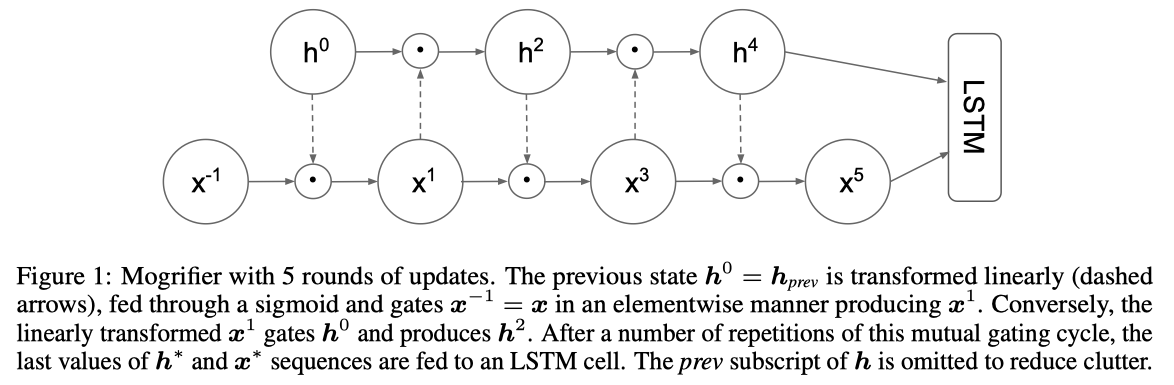
\includegraphics[scale=0.4]{images/MogrifierLSTM.png}
  \caption{Mogrifier LSTM.}
  \label{fig1}
\end{figure}

Mogrifier($\boldsymbol{x}, \boldsymbol{c}_{\text{prev}}, \boldsymbol{h}_{\text{prev}}$) =
LSTM($\boldsymbol{x}^\uparrow, \boldsymbol{c}_{\text{prev}}^{\uparrow}, \boldsymbol{h}_{\text{prev}}^{\uparrow}$).
$\boldsymbol{x}^\uparrow$ and $\boldsymbol{h}_{\text{prev}}^{\uparrow}$ are
defined as the highest indexed $x^i$ and $\boldsymbol{h}^{i}_{\text{prev}}$ as
in equation(\ref{eq1}) and (\ref{eq2}), where $\boldsymbol{x}^{-1} = \boldsymbol{x}$
and $\boldsymbol{h}_{\text{prev}}^{0} = \boldsymbol{h}_{\text{prev}}$, $r \in \mathbb{R}$
is a hyperparameter. $r = 0$ recovers LSTM.

\begin{eqnarray}
%\begin{aligned}
\boldsymbol{x}^i &= 2\sigma(\boldsymbol{Q}^i\boldsymbol{h}_{\text{prev}}^{i-1})
\odot \boldsymbol{x}^{i-2}, \qquad \text{for odd  } i \in [1\dotsc r] \label{eq1}\\
\boldsymbol{h}^i_{\text{prev}} &= 2\sigma(\boldsymbol{R}^i\boldsymbol{x}^{i-1})
\odot \boldsymbol{h}^{i-2}_{\text{prev}}, \qquad \text{for even  } i \in [1\dotsc r] \label{eq2}
%\end{aligned}
\end{eqnarray}

\section{Compare with other RNNs}

Input Switched Affine Network \cite{foerster2017input};
Hypernetworks \cite{ha2016hypernetworks};
Multiplicative LSTM\cite{krause2016multiplicative};


{
\small
\raggedright
\bibliographystyle{ieeetr}
% or, abbrv, acm, alpha, apalike, ieeetr, plain, siam, unsrt
\begin{spacing}{1}
\bibliography{references.bib}
\end{spacing}
}
\end{document}
